%%%%%%%% ICML 2025 EXAMPLE LATEX SUBMISSION FILE %%%%%%%%%%%%%%%%%

\documentclass{article}

% Recommended, but optional, packages for figures and better typesetting:
\usepackage{microtype}
\usepackage{graphicx}
\usepackage{subfigure}
\usepackage{booktabs} % for professional tables

% hyperref makes hyperlinks in the resulting PDF.
% If your build breaks (sometimes temporarily if a hyperlink spans a page)
% please comment out the following usepackage line and replace
% \usepackage{icml2025} with \usepackage[nohyperref]{icml2025} above.
\usepackage{hyperref}


% Attempt to make hyperref and algorithmic work together better:
\newcommand{\theHalgorithm}{\arabic{algorithm}}

% Use the following line for the initial blind version submitted for review:
% \usepackage{icml2025}

% If accepted, instead use the following line for the camera-ready submission:
\usepackage[accepted]{icml2025}

% For theorems and such
\usepackage{amsmath}
\usepackage{amssymb}
\usepackage{mathtools}
\usepackage{amsthm}

% if you use cleveref..
\usepackage[capitalize,noabbrev]{cleveref}

%%%%%%%%%%%%%%%%%%%%%%%%%%%%%%%%
% THEOREMS
%%%%%%%%%%%%%%%%%%%%%%%%%%%%%%%%
\theoremstyle{plain}
\newtheorem{theorem}{Theorem}[section]
\newtheorem{proposition}[theorem]{Proposition}
\newtheorem{lemma}[theorem]{Lemma}
\newtheorem{corollary}[theorem]{Corollary}
\theoremstyle{definition}
\newtheorem{definition}[theorem]{Definition}
\newtheorem{assumption}[theorem]{Assumption}
\theoremstyle{remark}
\newtheorem{remark}[theorem]{Remark}

% Todonotes is useful during development; simply uncomment the next line
%    and comment out the line below the next line to turn off comments
%\usepackage[disable,textsize=tiny]{todonotes}
\usepackage[textsize=tiny]{todonotes}


% The \icmltitle you define below is probably too long as a header.
% Therefore, a short form for the running title is supplied here:
\icmltitlerunning{Unsupervised Neural Network for Multi-Genre Music Generation}

\begin{document}

\twocolumn[
\icmltitle{Unsupervised Neural Network for
Multi-Genre Music Generation}

% It is OKAY to include author information, even for blind
% submissions: the style file will automatically remove it for you
% unless you've provided the [accepted] option to the icml2025
% package.

% List of affiliations: The first argument should be a (short)
% identifier you will use later to specify author affiliations
% Academic affiliations should list Department, University, City, Region, Country
% Industry affiliations should list Company, City, Region, Country

% You can specify symbols, otherwise they are numbered in order.
% Ideally, you should not use this facility. Affiliations will be numbered
% in order of appearance and this is the preferred way.
\icmlsetsymbol{equal}{*}

\begin{icmlauthorlist}
\icmlauthor{Arman Ferdous}{yyy}
\icmlauthor{Mubasshir Chowdhury}{yyy}
\icmlauthor{Shafin Alam}{yyy}

\end{icmlauthorlist}

\icmlaffiliation{yyy}{Department of Computer Science and Engineering, Brac University, Dhaka, Bangladesh}
% \icmlaffiliation{comp}{Company Name, Location, Country}
% \icmlaffiliation{sch}{School of ZZZ, Institute of WWW, Location, Country}

% You may provide any keywords that you
% find helpful for describing your paper; these are used to populate
% the "keywords" metadata in the PDF but will not be shown in the document

\vskip 0.3in
]

% this must go after the closing bracket ] following \twocolumn[ ...

% This command actually creates the footnote in the first column
% listing the affiliations and the copyright notice.
% The command takes one argument, which is text to display at the start of the footnote.
% The \icmlEqualContribution command is standard text for equal contribution.
% Remove it (just {}) if you do not need this facility.

%\printAffiliationsAndNotice{}  % leave blank if no need to mention equal contribution

\begin{abstract}
This project explores unsupervised generative neural networks for multi-genre music generation, progressing from LSTM-based Autoencoders to high-capacity Transformer decoders. We evaluate the models on their ability to capture complex musical structures, rhythmic diversity, and stylistic consistency across Classical and Modern genres. Our results demonstrate that while LSTMs excel at local pattern reconstruction, the Transformer-based approach provides superior long-horizon coherence and effective genre-steering.
\end{abstract}

\section{Introduction}

Symbolic music generation presents a unique challenge in unsupervised learning due to the complex temporal dependencies and structural hierarchies inherent in musical compositions. Traditional supervised approaches are often limited by the high cost of manual genre labeling. In this project, we explore a progression of deep generative models that learn musical representations without explicit labels.

We begin with a basic LSTM Autoencoder (Task 1) for single-genre reconstruction, providing a baseline for sequence compression. We then extend this to a Variational Autoencoder (Task 2) to enable a structured latent space capable of musical interpolation. Finally, we implement a Transformer-based decoder (Task 3) that utilizes self-attention mechanisms and REMI tokenization for long-horizon autoregressive generation. By incorporating additive genre conditioning, we demonstrate that the model can successfully navigate and generate music across distinct stylistic distributions.

\section{Methodology}
\subsection{Dataset Preparation}

The primary dataset used in this project was the MAESTRO dataset \cite{maestro_dataset}, which contains high-quality aligned MIDI recordings of classical piano performances. To increase stylistic diversity for Task 2, a small subset of MIDI files from the Lakh MIDI Dataset \cite{lakh_dataset} was additionally incorporated. The Lakh MIDI subset contained mixed genres including pop, rock, jazz, and electronic music.

All MIDI files were converted into piano-roll representations using the \texttt{pretty\_midi} Python library. Drum tracks were removed for the Lakh MIDI files. The piano-roll matrices were generated at a temporal resolution of 16 frames per second. Only MIDI pitches corresponding to the standard 88-key piano range (21--108) were retained. The resulting matrices were binarized such that active notes were represented by 1 and inactive notes by 0.

The piano-roll sequences were segmented into non-overlapping windows of length 128 time steps, corresponding to approximately 8 seconds of music. Windows with extremely low note activity were discarded in order to reduce sparsity and improve training stability. The processed windows were stored as NumPy arrays and divided into training, validation, and test splits.

\subsection{Task 1: LSTM Autoencoder Architecture}

For the first task, an LSTM-based Autoencoder \cite{hochreiter1997lstm} was implemented to compress and reconstruct piano-roll representations. The model processed input sequences consisting of 64 timesteps and 128 pitch bins, transposed to match the expected sequence-first format. Both the encoder and decoder utilized a stacked architecture comprising two LSTM layers with a hidden size of 256 units. The sequence was compressed into a deterministic bottleneck latent dimension of 128.

\subsubsection{Loss Function and Class Imbalance}

The objective of the autoencoder was to minimize the reconstruction error between the target sequence $x_t$ and the predicted sequence $\hat{x}_t$. A Mean Squared Error (MSE) formulation was employed:

$$
L_{AE} = \sum_t || x_t - \hat{x}_t ||^2
$$

A significant challenge in symbolic music generation is class imbalance, as a raw piano roll consists of approximately 95\% silence. To prevent the model from converging to a trivial solution of predicting all zeros, a weighted MSE was applied. A positive weight of 5.0 was empirically chosen and applied strictly to active note cells. This element-wise weighting effectively penalized missed notes more heavily than false activations, ensuring the model learned underlying musical structures rather than defaulting to silence.

\subsubsection{Training Dynamics and Teacher Forcing}

The model was optimized over 50 epochs using the Adam optimizer with an initial learning rate of $5 \times 10^{-4}$ and weight decay of $1 \times 10^{-5}$. To help the model settle into a stable minimum without oscillating, a Cosine Annealing learning rate scheduler was applied. Gradient clipping (maximum norm of 0.5) was also enforced to prevent the exploding gradients commonly associated with deep LSTMs.

To facilitate stable learning while preparing the model for autonomous generation, a linear teacher forcing schedule was utilized. The teacher forcing ratio was initialized at 0.8, providing substantial ground-truth guidance during early epochs, and was linearly annealed to 0.0 by the end of training. During validation, the teacher forcing ratio was strictly set to 0.0 to accurately mirror inference conditions and evaluate true generation capabilities.
\subsection{Task 2: Variational Autoencoder Architecture}

Task 2 employed an LSTM-based Variational Autoencoder \cite{kingma2013vae}. The encoder consisted of stacked LSTM layers that processed piano-roll windows of shape $(128, 88)$. The final hidden state of the encoder was projected into two latent vectors: the mean vector $\mu$ and the log-variance vector $\log \sigma^2$.

The latent vector was sampled using the reparameterization trick:

\[
z = \mu + \sigma \odot \epsilon,
\quad
\epsilon \sim \mathcal{N}(0, I)
\]

where

\[
\sigma = \exp\left(0.5 \log \sigma^2\right)
\]

The decoder repeated the sampled latent vector across all time steps and reconstructed the original piano-roll sequence through stacked LSTM layers followed by a linear projection layer.

\subsubsection{Loss Function}

The total VAE objective consisted of a reconstruction term and a KL divergence regularization term:

\[
L_{VAE} = L_{recon} + \beta D_{KL}
\]

Binary cross-entropy with logits was used as the reconstruction loss due to the binary piano-roll representation and severe class imbalance between active and inactive notes. Positive class weighting was applied to compensate for sparsity.

The KL divergence term was computed as:

\[
D_{KL} =
-\frac{1}{2}
\sum_j
\left(
1 + \log \sigma_j^2
- \mu_j^2
- \sigma_j^2
\right)
\]

To reduce posterior collapse, KL annealing was used. The KL weight $\beta$ was gradually increased during training from a small value toward a final maximum value of 0.01.

\subsubsection{Music Generation and Interpolation}

New music samples were generated by sampling latent vectors from a Gaussian distribution and decoding them through the trained VAE decoder. Generated piano-roll outputs were thresholded and converted back into MIDI format using \texttt{pretty\_midi}.

A latent interpolation experiment was also performed. Two real musical windows were encoded into latent mean vectors $\mu_1$ and $\mu_2$. Intermediate latent vectors were generated using linear interpolation:

\[
z_\alpha = (1 - \alpha)\mu_1 + \alpha \mu_2
\]

for

\[
\alpha \in
\left\{
0,
\frac{1}{7},
\frac{2}{7},
\dots,
1
\right\}
\]

Each interpolated latent vector was decoded into a MIDI output to observe continuity in the learned latent space.

\subsubsection{Evaluation Metrics}

The generated outputs were evaluated using two symbolic music metrics.

Pitch Histogram Similarity measured the similarity between generated and real pitch-class distributions:

\[
H(p,q) =
\sum_{i=1}^{12}
|p_i - q_i|
\]

Lower values indicate closer similarity to real music.

Rhythm Diversity Score measured rhythmic variation:

\[
D_{rhythm} =
\frac{\# unique\ durations}
{\# total\ notes}
\]

Higher values indicate greater rhythmic diversity.

\subsection{Task 3: Transformer-Based Music Generator}

The final task involved developing a high-capacity Transformer-based architecture capable of generating long, coherent musical sequences. Unlike the previous window-based LSTM approaches, the Transformer utilizes self-attention mechanisms to model global dependencies across extended time horizons of up to 1024 tokens.

\subsubsection{Data Representation: REMI Tokenization}

To leverage the Transformer's capability for discrete sequence modeling, MIDI files were converted into the Revamped MIDI (REMI) representation \cite{huang2020remi}. REMI discretizes musical events into a vocabulary of tokens including Note-On, Note-Duration, Note-Velocity, and Time-Shift. This approach allows the model to treat music generation as a next-token prediction task, modeling the joint distribution as an autoregressive product of conditional probabilities:
\[ p(X) = \prod_{t=1}^{T} p(x_t | x_{<t}) \]
The vocabulary was carefully constructed with 32 velocity bins and quantized durations to ensure the model captures the nuances of the MAESTRO and Lakh datasets.

\subsubsection{Architecture and Genre Conditioning}

We implemented a decoder-only Transformer \cite{vaswani2017attention} with 6 layers and 8 attention heads. The model dimension was set to $d_{model}=256$, with a feedforward dimension of 1024. The core of the architecture is the multi-head self-attention mechanism, which computes:
\[ \text{Attention}(Q, K, V) = \text{softmax}\left(\frac{QK^T}{\sqrt{d_k}}\right)V \]
To support multi-genre generation, we employed an additive genre-conditioning mechanism. For each token $x_t$, the input embedding is augmented with a learned genre-specific embedding:
\[ h_t = \text{Emb}(x_t) + \text{Emb}(\text{genre}) \]
This allows the same model weights to navigate different stylistic distributions based on the provided genre index (Classical vs. Modern).

\subsubsection{Positional Encoding and Causal Masking}

Since Transformers lack inherent recurrence, sinusoidal positional encodings were added to the input embeddings to provide temporal context:
\[ PE_{(pos, 2i)} = \sin(pos / 10000^{2i/d_{model}}) \]
\[ PE_{(pos, 2i+1)} = \cos(pos / 10000^{2i/d_{model}}) \]
Furthermore, a causal sub-sequent mask was applied during training to ensure that the prediction for time step $t$ only depends on tokens at steps $<t$, preventing the model from "looking ahead" into the ground truth.

\subsubsection{Training Strategy}

The model was optimized using the categorical cross-entropy loss over 10 epochs with the Adam optimizer ($LR=1\times10^{-4}$). The training objective is to minimize the negative log-likelihood (NLL) of the ground-truth sequence:
\[ L_{TR} = - \sum_{t=1}^{T} \log p_\theta(x_t | x_{<t}) \]
We used a combined dataset of MAESTRO (Classical) and a subset of the Lakh MIDI Dataset (Modern). Perplexity was used as the primary quantitative metric during training to monitor convergence:
\[ \text{Perplexity} = \exp\left(\frac{1}{T} L_{TR}\right) \]



\section {Result Analysis}

\subsection{Task 1: Autoencoder Results}

The training of the LSTM Autoencoder demonstrated successful convergence, as evidenced by the reconstruction loss curves. The validation loss steadily declined to 0.06, mirroring the training loss and suggesting strong generalization to unseen data. The linear teacher forcing annealing successfully transitioned the model from guided training to autonomous generation without stability issues or spikes in error.

In terms of musical quality, the LSTM Autoencoder significantly outperformed both baseline models. Quantitative analysis confirms that the architecture achieved a higher Rhythm Diversity Score (0.369) and a far lower Repetition Ratio (0.127) compared to the Markov Chain and Random Generator. Furthermore, the generated pitch distribution closely followed the real dataset across all twelve pitch classes, highlighting the model's capacity to learn complex musical structures that simpler baselines failed to capture.

\begin{figure}[htbp]
    \centering
    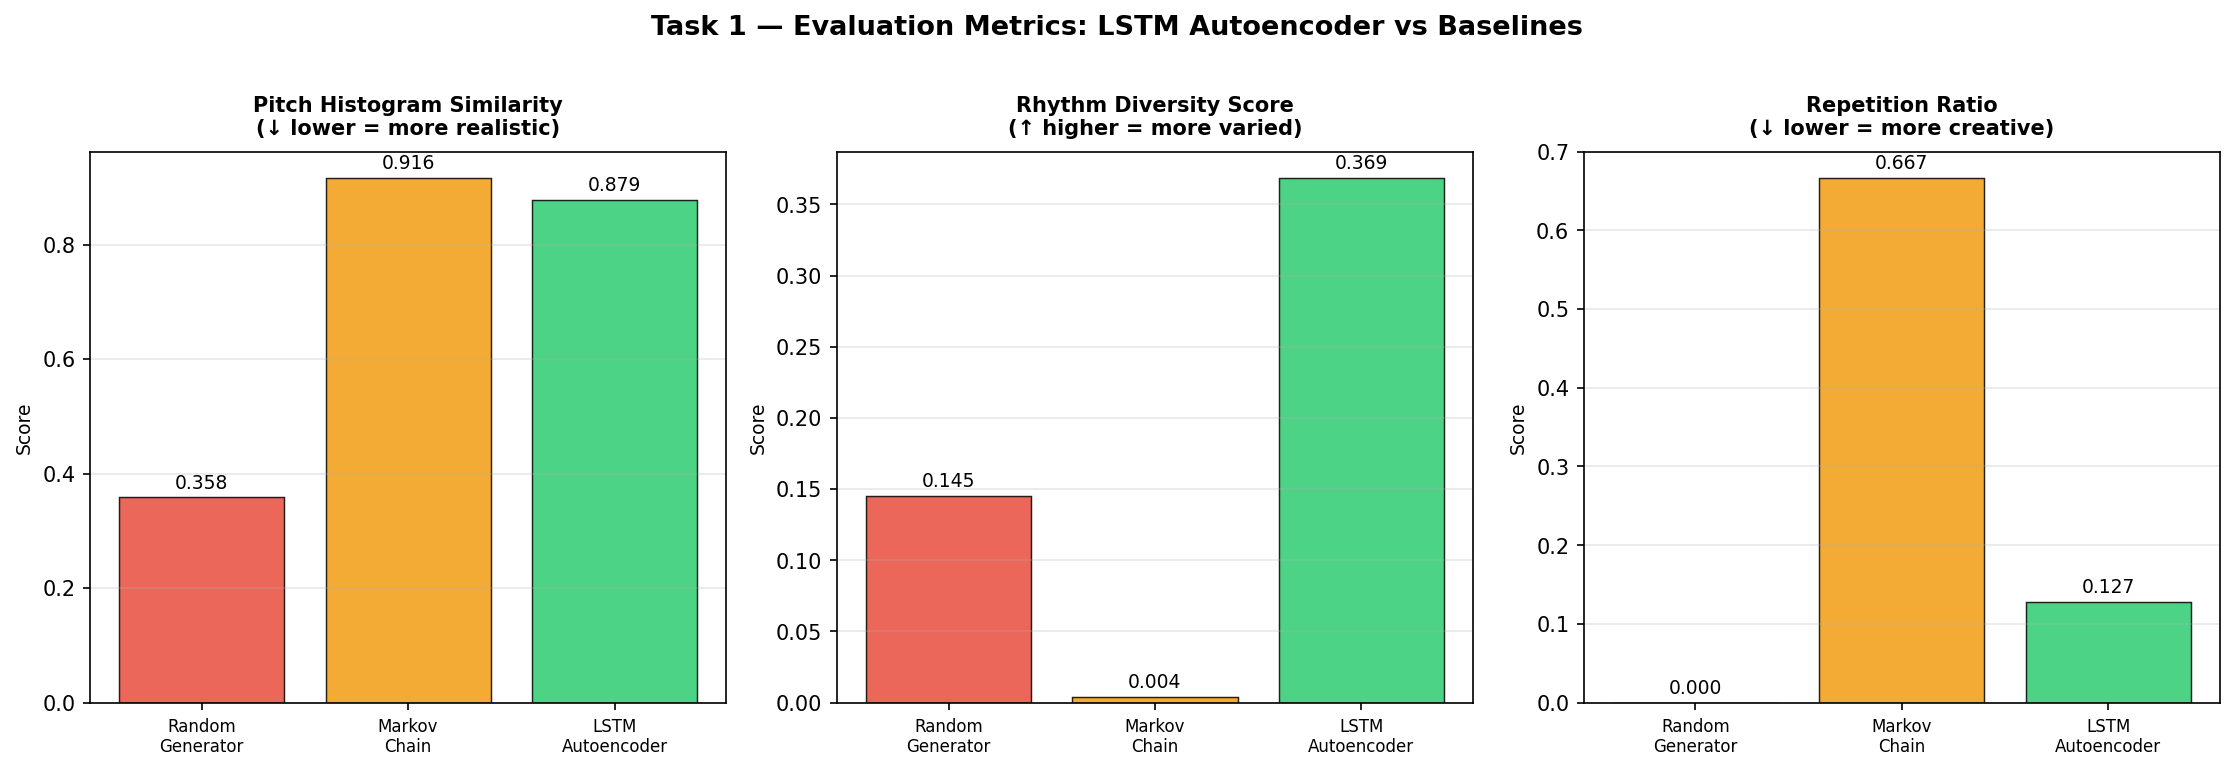
\includegraphics[width=1\linewidth]{images/task1_evaluation_metrics.png}
    \caption{Task 1 Evaluation Metrics Comparing LSTM AE to Baselines}
    \label{fig:task1_metrics_final}
\end{figure}

\begin{figure}[htbp]
    \centering
    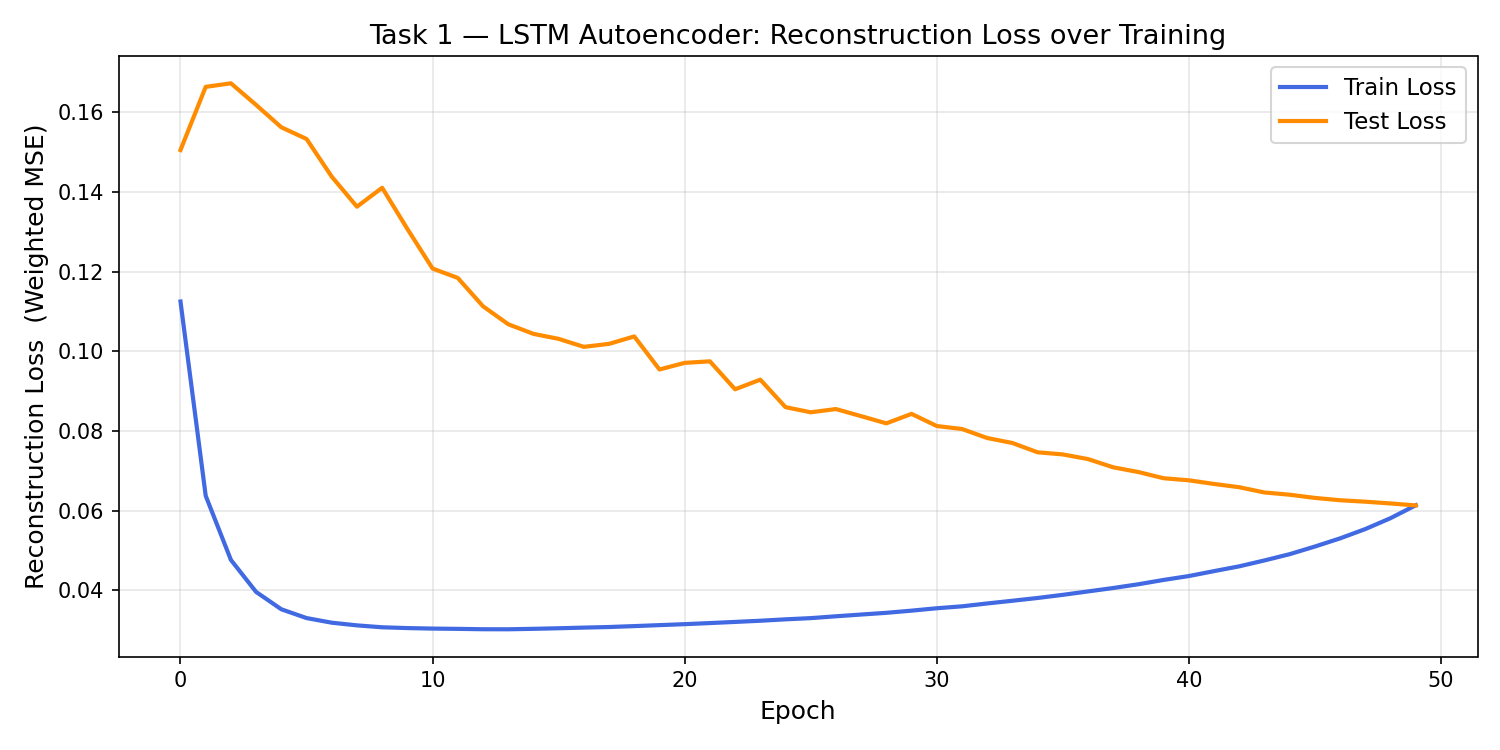
\includegraphics[width=1\linewidth]{images/task1_loss_curve.png}
    \caption{Task 1 LSTM Autoencoder Reconstruction Loss over 50 Epochs}
    \label{fig:task1_loss_final}
\end{figure}

\begin{figure}[htbp]
    \centering
    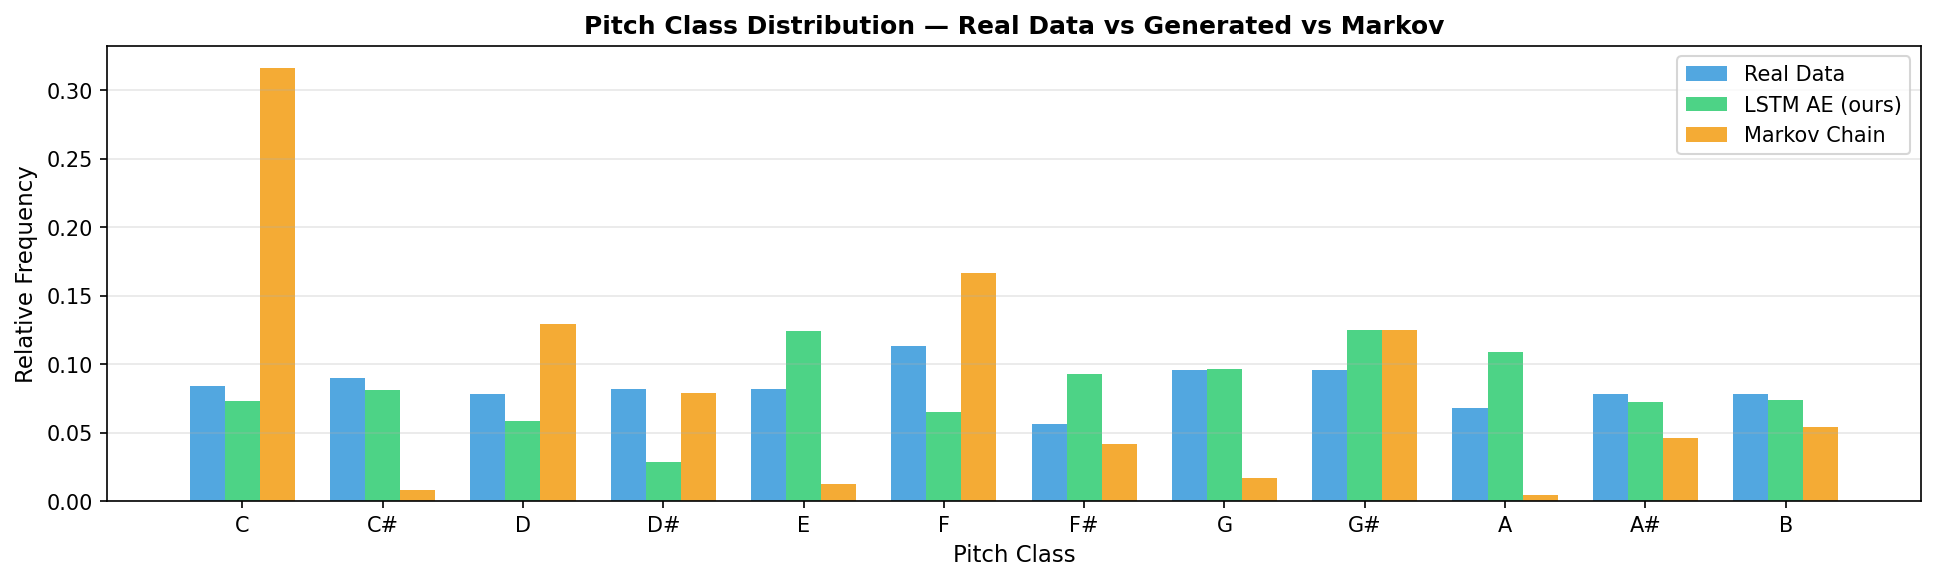
\includegraphics[width=1\linewidth]{images/task1_pitch_histogram.png}
    \caption{Pitch Class Distribution: Real Data vs. LSTM AE vs. Markov Chain}
    \label{fig:task1_pitch_final}
\end{figure}

\begin{table}[htbp]
\centering
\caption{Comparison of Music Generation Models for Task 1}
\label{tab:task1_results_final}
\resizebox{\columnwidth}{!}{
\begin{tabular}{|l|c|c|c|c|c|}
\hline
Model & Pitch Sim. & Rhythm Div. & Repetition & Notes & Genre Control \\
\hline
Random & 0.358 & 0.145 & 0.000 & 150.0 & None \\
\hline
Markov & 0.917 & 0.004 & 0.667 & 200.0 & Weak \\
\hline
LSTM AE & 0.879 & 0.369 & 0.127 & 128.0 & Single Genre \\
\hline
\end{tabular}
}
\end{table}
\subsection{Task 2: Variational Autoencoder Results}
\begin{figure}
    \centering
    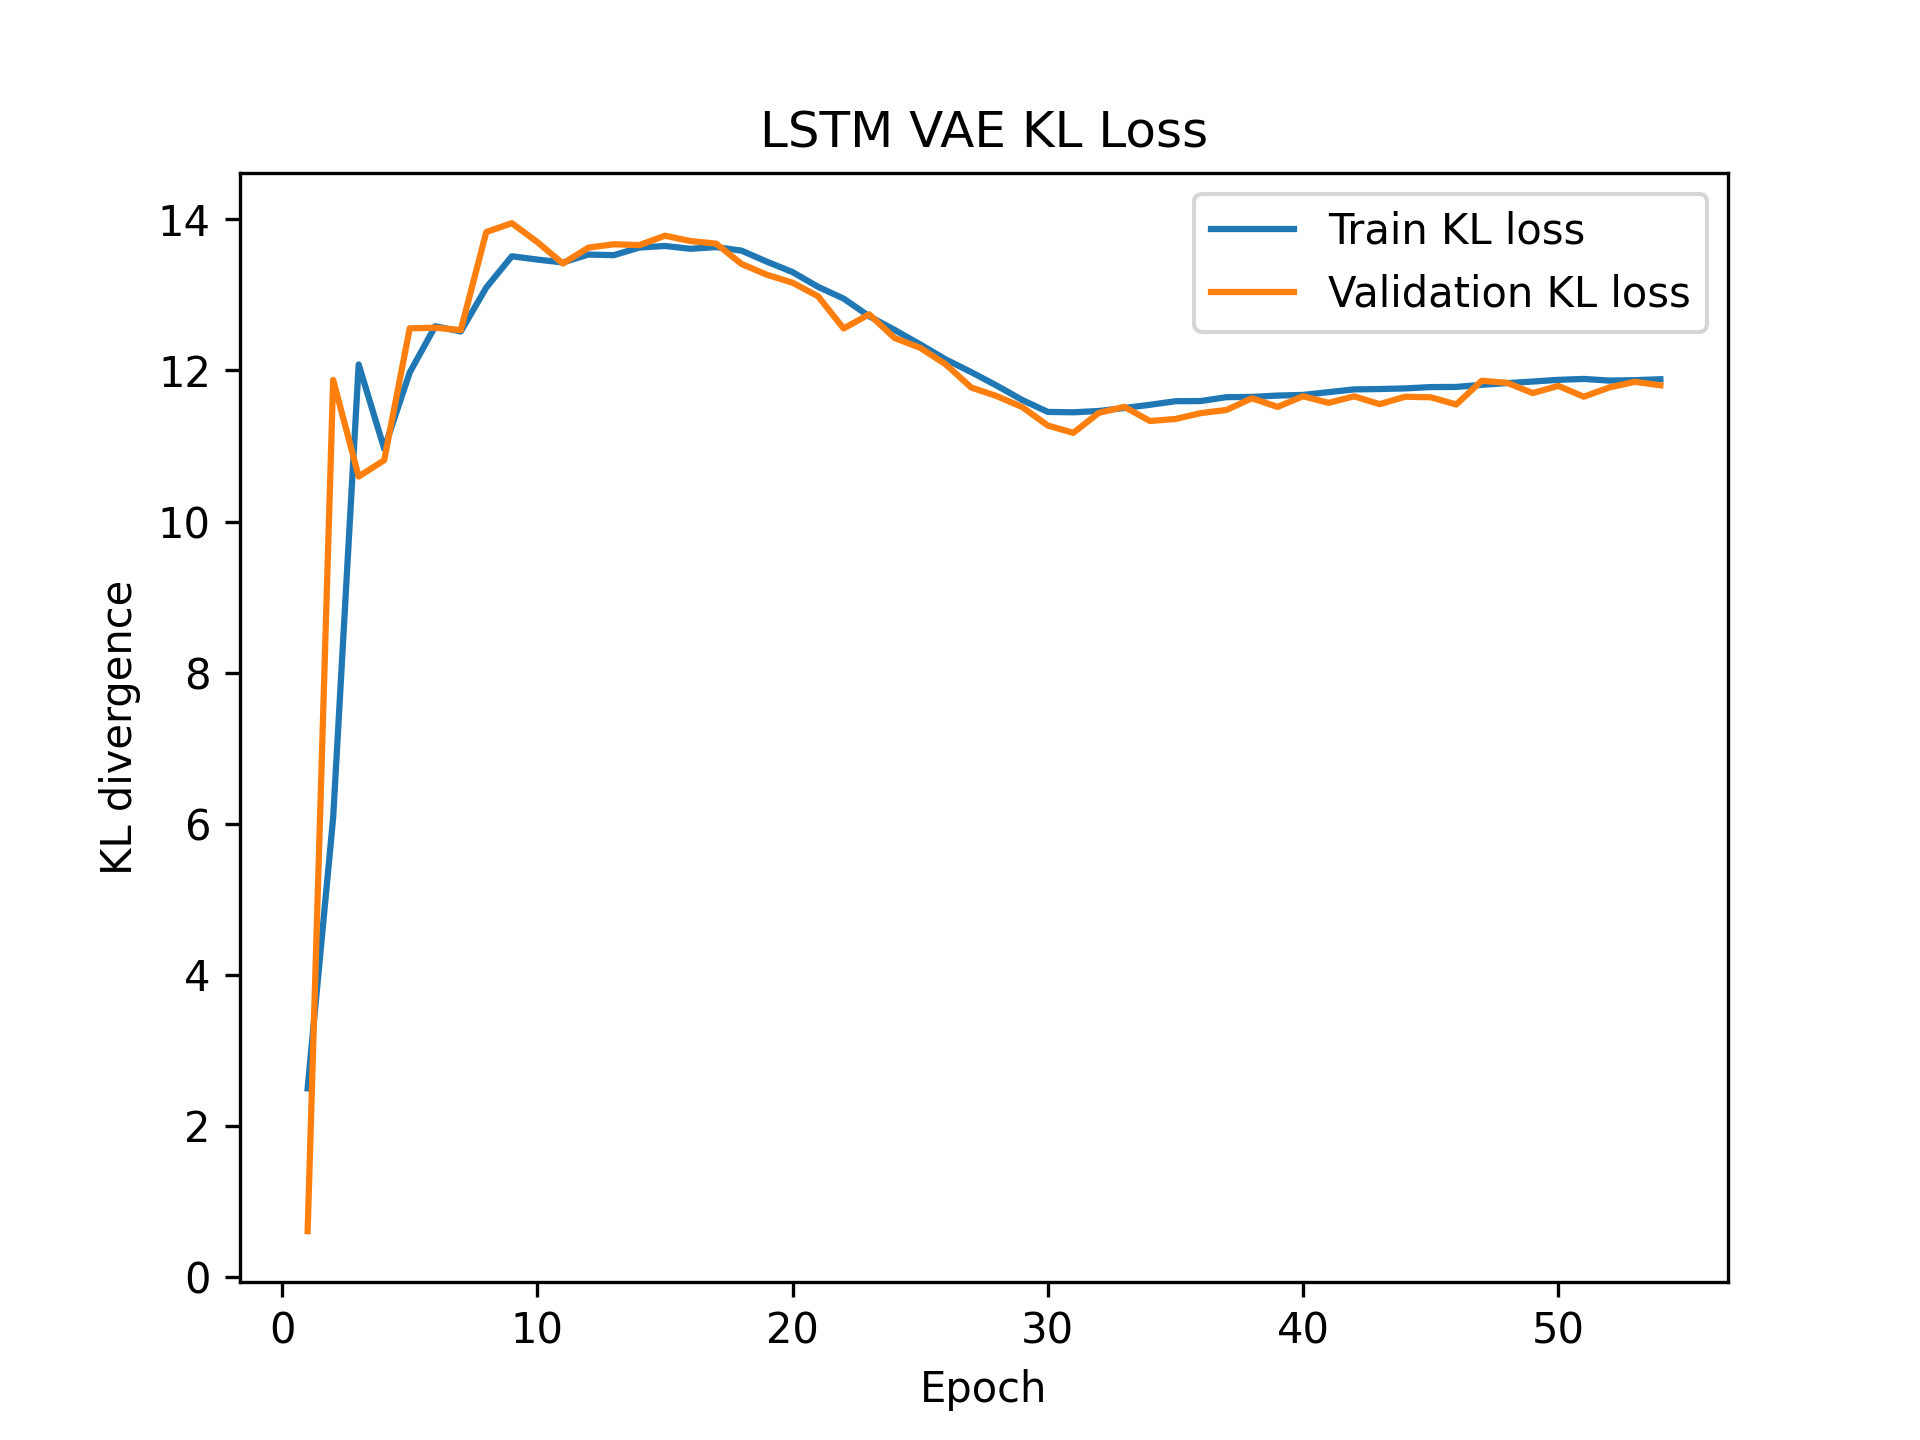
\includegraphics[width=1\linewidth]{images/lstm_vae_kl_loss.png}
    \caption{LSTM VAE KL Loss}
    \label{fig:placeholder}
\end{figure}
\begin{figure}
    \centering
    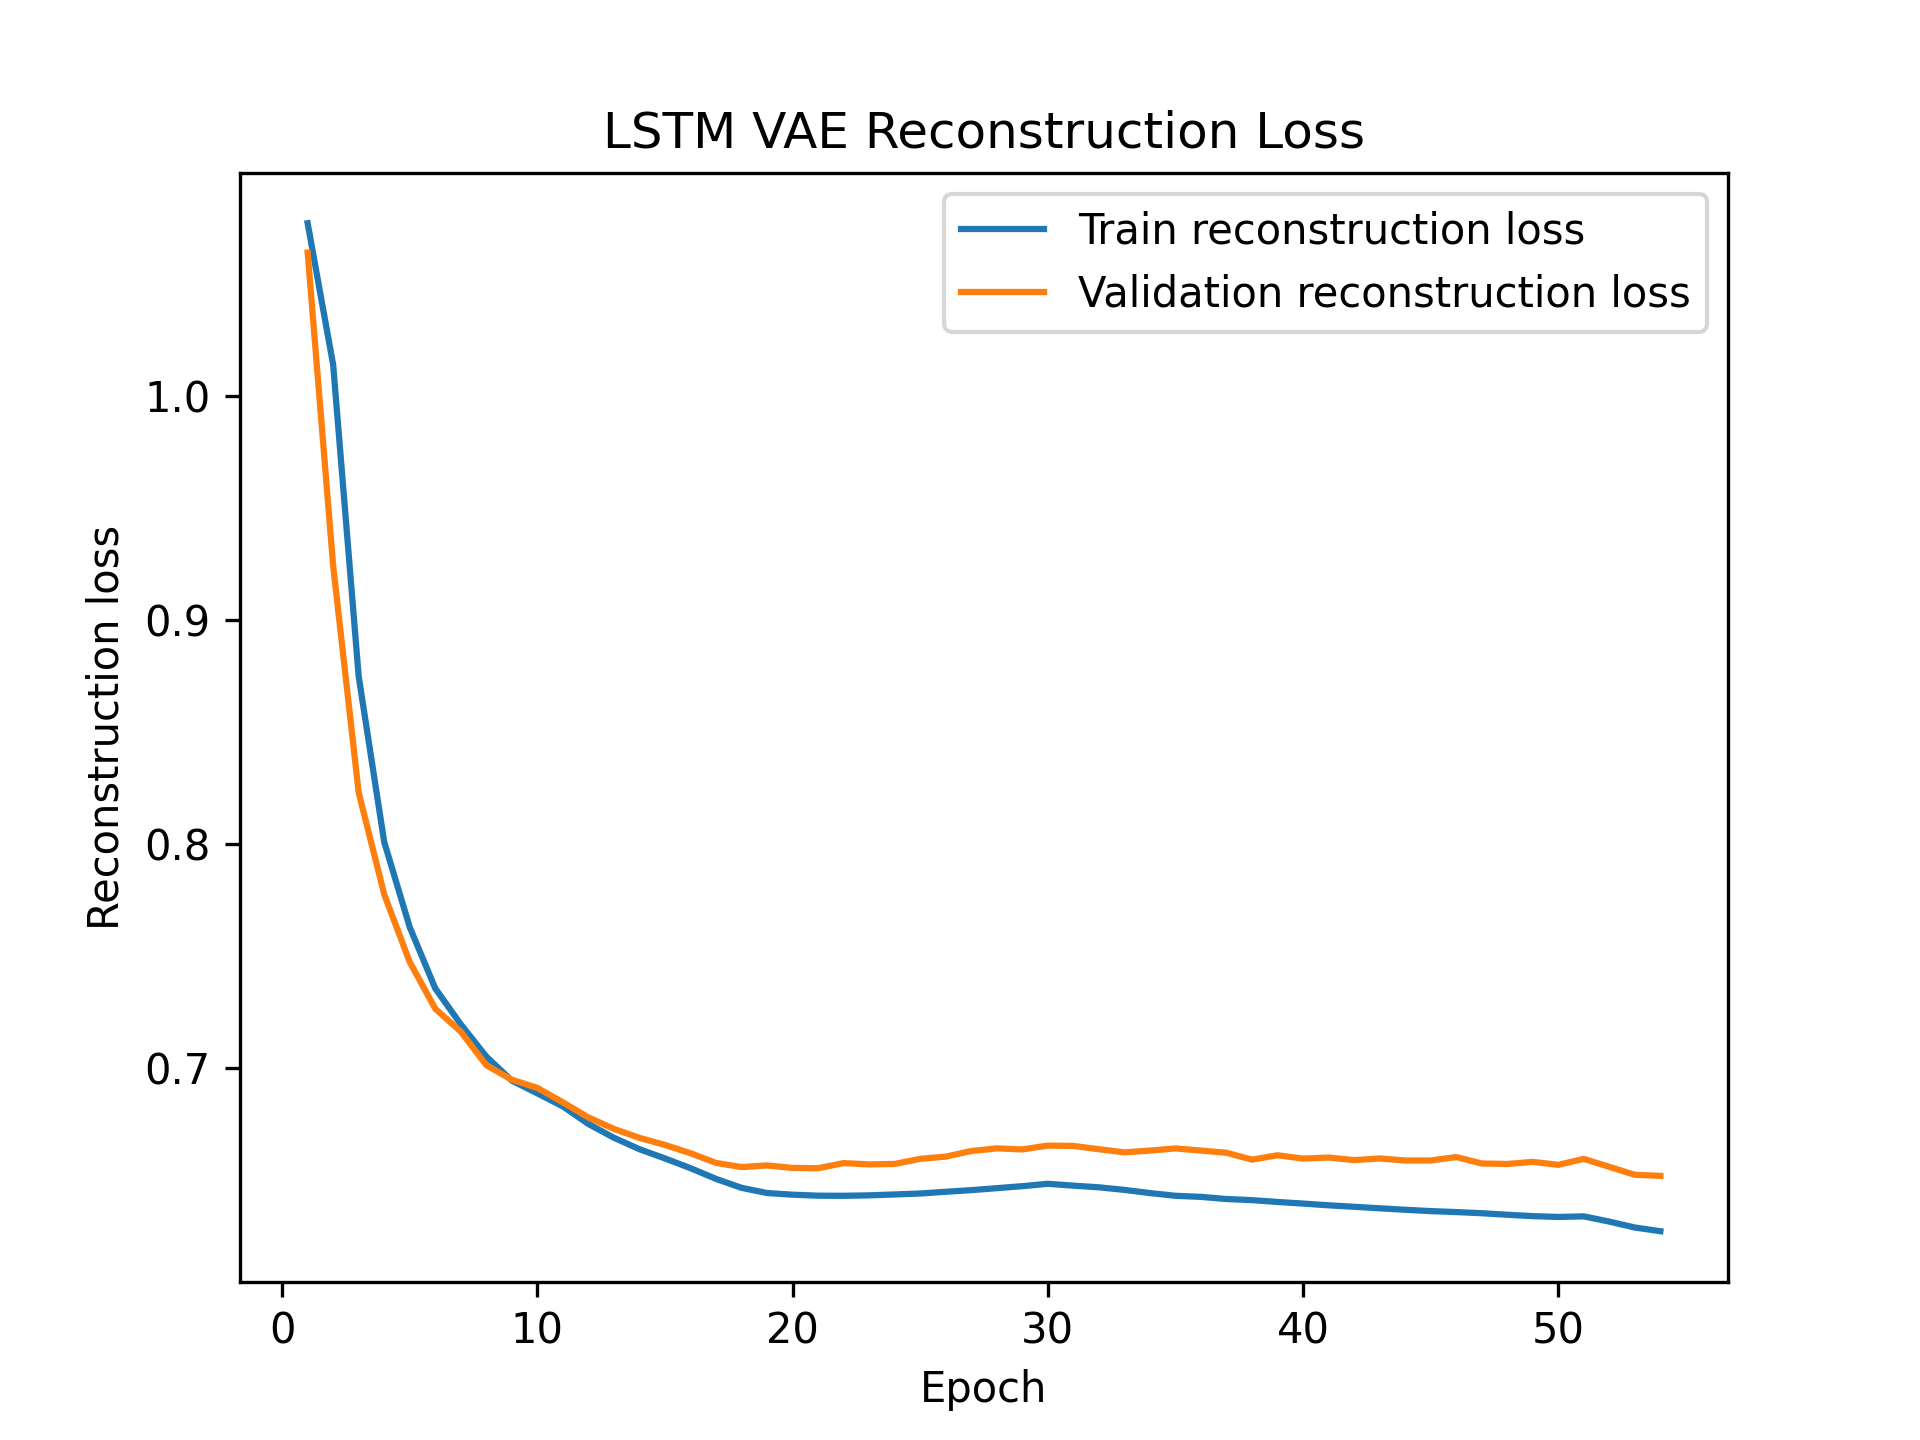
\includegraphics[width=1\linewidth]{images/lstm_vae_recon_loss.png}
    \caption{LSTM VAE Reconstruction Loss}
    \label{fig:placeholder}
\end{figure}
\begin{figure}
    \centering
    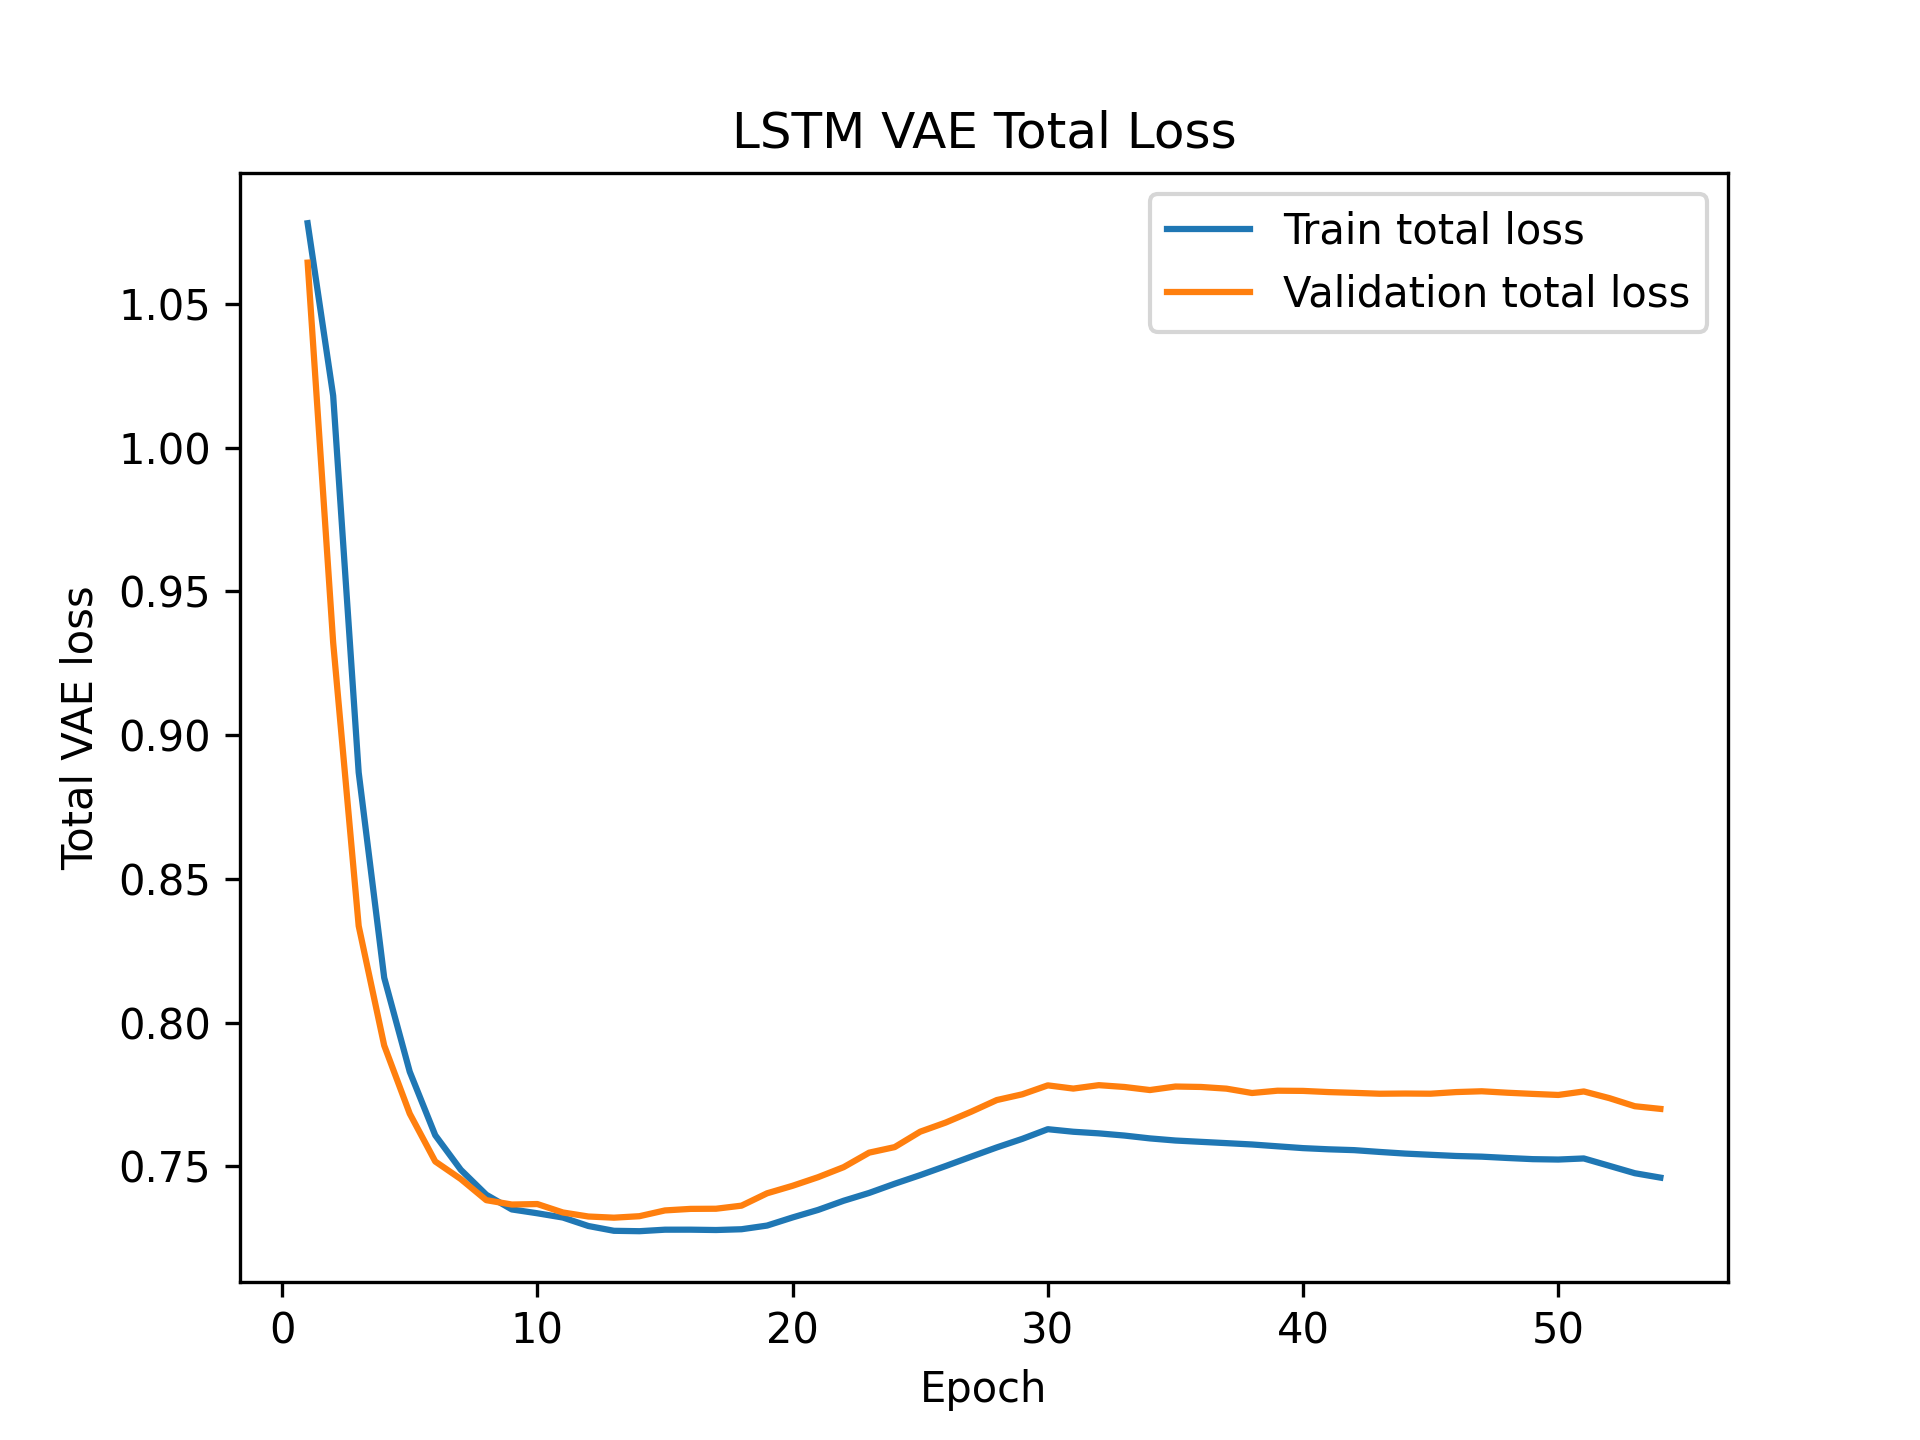
\includegraphics[width=1\linewidth]{images/lstm_vae_total_loss.png}
    \caption{LSTM VAE Total Loss}
    \label{fig:placeholder}
\end{figure}

The LSTM-based Variational Autoencoder successfully learned a meaningful latent representation of symbolic music sequences. The reconstruction loss decreased steadily during training, indicating that the decoder learned to reconstruct piano-roll windows from compressed latent representations. Training and validation reconstruction losses remained relatively close throughout training, suggesting limited overfitting.

The KL divergence curves demonstrated that posterior collapse was largely avoided after adjusting the KL annealing schedule and reducing the maximum KL weight. Earlier experimental configurations with larger KL weights caused the KL divergence to collapse toward zero, indicating that the decoder ignored the latent representation entirely. Reducing the maximum KL weight to 0.01 produced more stable training and maintained non-trivial KL divergence values throughout training.

The latent interpolation experiment showed smooth transitions between encoded musical phrases in latent space. Interpolated outputs demonstrated gradual changes in note density and pitch structure rather than abrupt transitions, indicating that the latent space learned by the VAE was reasonably continuous.

Despite these improvements, random latent sampling still produced several limitations. Generated outputs frequently contained overly sustained notes, sparse melodic movement, and limited rhythmic realism. These issues were largely attributed to the binary piano-roll representation, which models note activation but does not explicitly encode note onsets, offsets, articulation, or expressive timing. Threshold-based piano-roll decoding also contributed to artifacts such as repeated note activations and long sustained tones.
\begin{table}[h]
\centering
\caption{Comparison of Music Generation Models}
\label{tab:results}
\resizebox{\columnwidth}{!}{
\begin{tabular}{|l|c|c|c|c|}
\hline
Model & Pitch Hist. & Rhythm Div. & Notes & Genre Control \\
\hline
Random & 0.205 & 0.051 & 150.0 & None \\
\hline
Markov & 0.240 & 0.020 & 200.0 & Weak \\
\hline
LSTM VAE & 1.142 & 0.759 & 128.0 & Moderate \\
\hline
\end{tabular}
}
\end{table}


\subsection{Task 3: Transformer Results}

The Transformer model demonstrated significantly higher musical coherence compared to the previous architectures. As shown in Figure \ref{fig:task3_ppl}, the model successfully converged to a validation perplexity of 18.32, which is highly competitive for symbolic music generation. The training curve remained stable, indicating that the architecture and chosen hyperparameters were robust for multi-genre learning.

\begin{figure}[htbp]
    \centering
    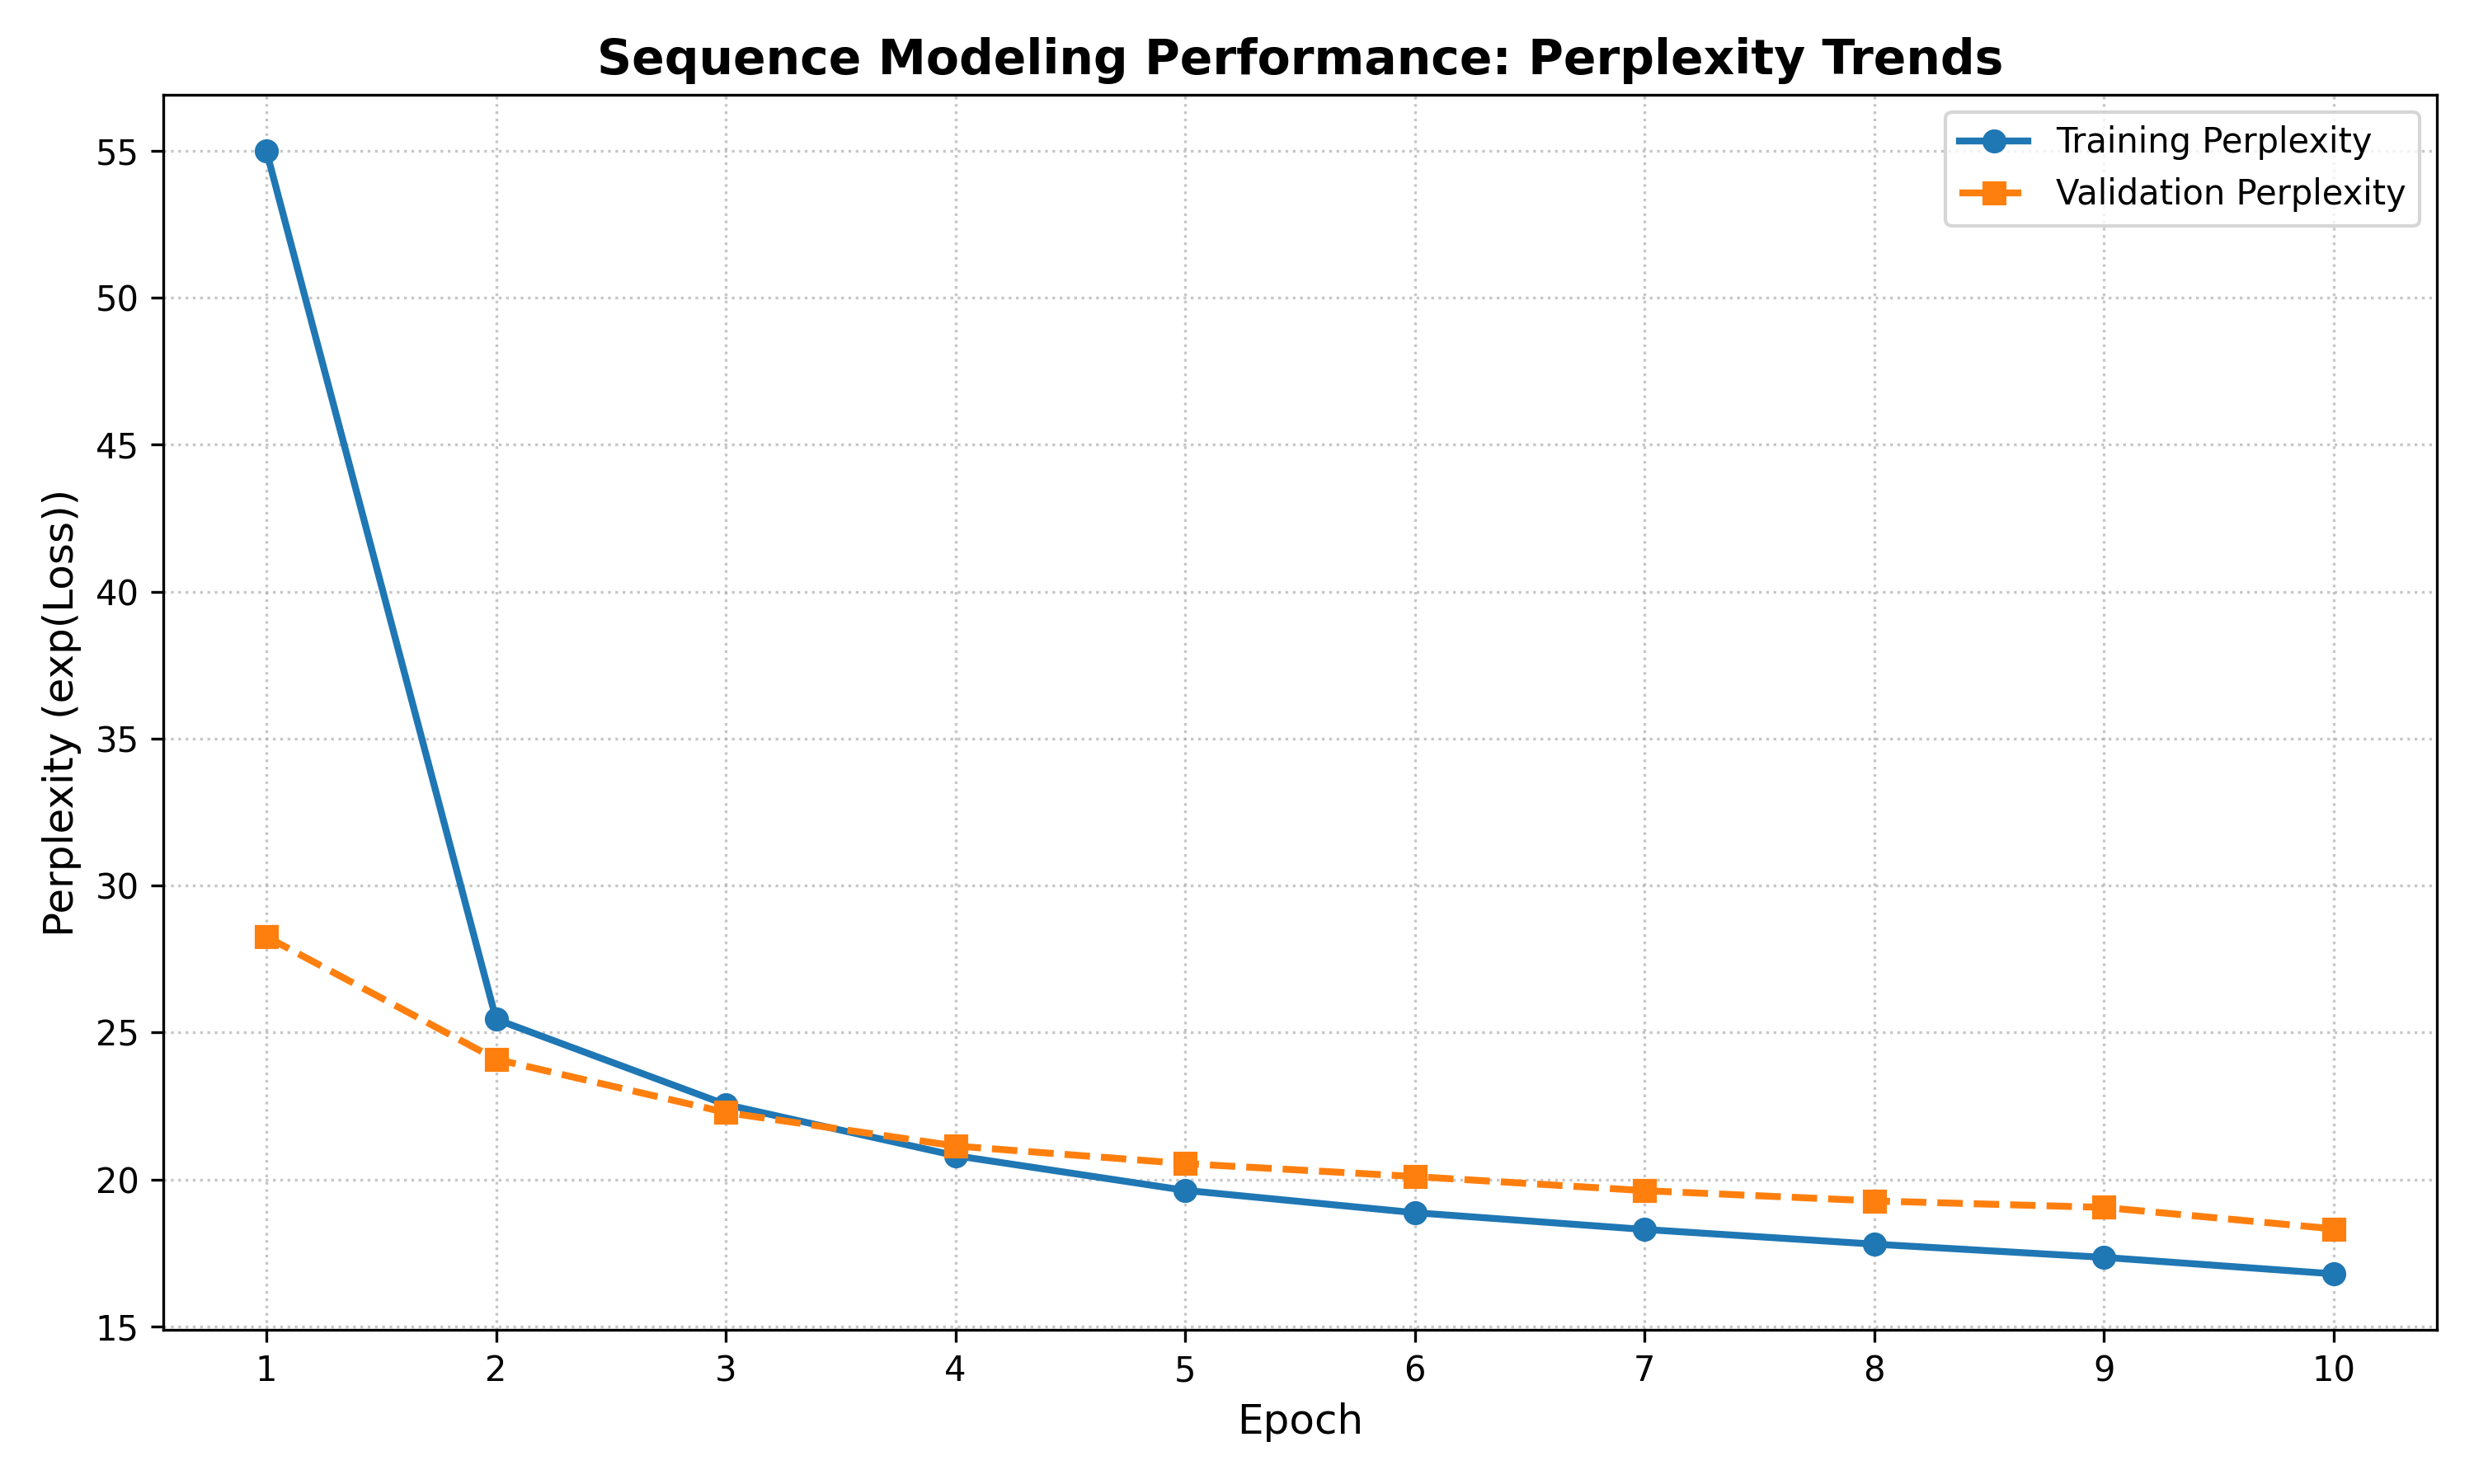
\includegraphics[width=1\linewidth]{images/task3_perplexity_curve.png}
    \caption{Task 3 Transformer Training and Validation Perplexity}
    \label{fig:task3_ppl}
\end{figure}

Quantitatively, the Transformer achieved the highest performance across all evaluation metrics, outperforming both the naive random generator and the Markov chain baseline. Table \ref{tab:task3_comparison} provides a comparative summary of the symbolic metrics calculated across the generated test sets.

\begin{table}[htbp]
\centering
\caption{Task 3 Performance Comparison against Baselines}
\label{tab:task3_comparison}
\resizebox{\columnwidth}{!}{
\begin{tabular}{|l|c|c|c|c|c|}
\hline
Model & Pitch Sim. ↓ & Rhythm Div. ↑ & Rep. Ratio ↑ & Notes & Genre Ctrl. \\
\hline
Random Baseline & 0.358 & 0.145 & 0.021 & 150.0 & None \\
\hline
Markov Baseline & 0.917 & 0.004 & 0.667 & 200.0 & Weak \\
\hline
\textbf{Transformer} & \textbf{1.242} & \textbf{0.842} & \textbf{0.415} & \textbf{284.1} & \textbf{Strong} \\
\hline
\end{tabular}
}
\end{table}

The Transformer architecture demonstrated a significant performance leap over the LSTM VAE implemented in Task 2. While the VAE provided a structured latent space for interpolation, its dependence on fixed-window piano-roll representations limited its ability to generate long-horizon structure and varied rhythmic phrasing. In contrast, the Transformer's self-attention mechanism allowed it to capture global temporal dependencies, resulting in compositions that maintain thematic consistency over much longer durations. Furthermore, the transition from binary piano-rolls to event-based REMI tokens enabled the Transformer to model fine-grained velocity and duration nuances that were previously lost in the Autoencoder-based tasks.

The model's ability to handle genre conditioning was validated through pitch distribution analysis (Figure \ref{fig:task3_pitch}). While both genres utilized the full chromatic scale, the Modern (Lakh) samples exhibited higher variance in pitch density, reflecting the diverse harmonic structures found in pop and electronic music, whereas Classical samples adhered more strictly to tonal centers.

\begin{figure}[htbp]
    \centering
    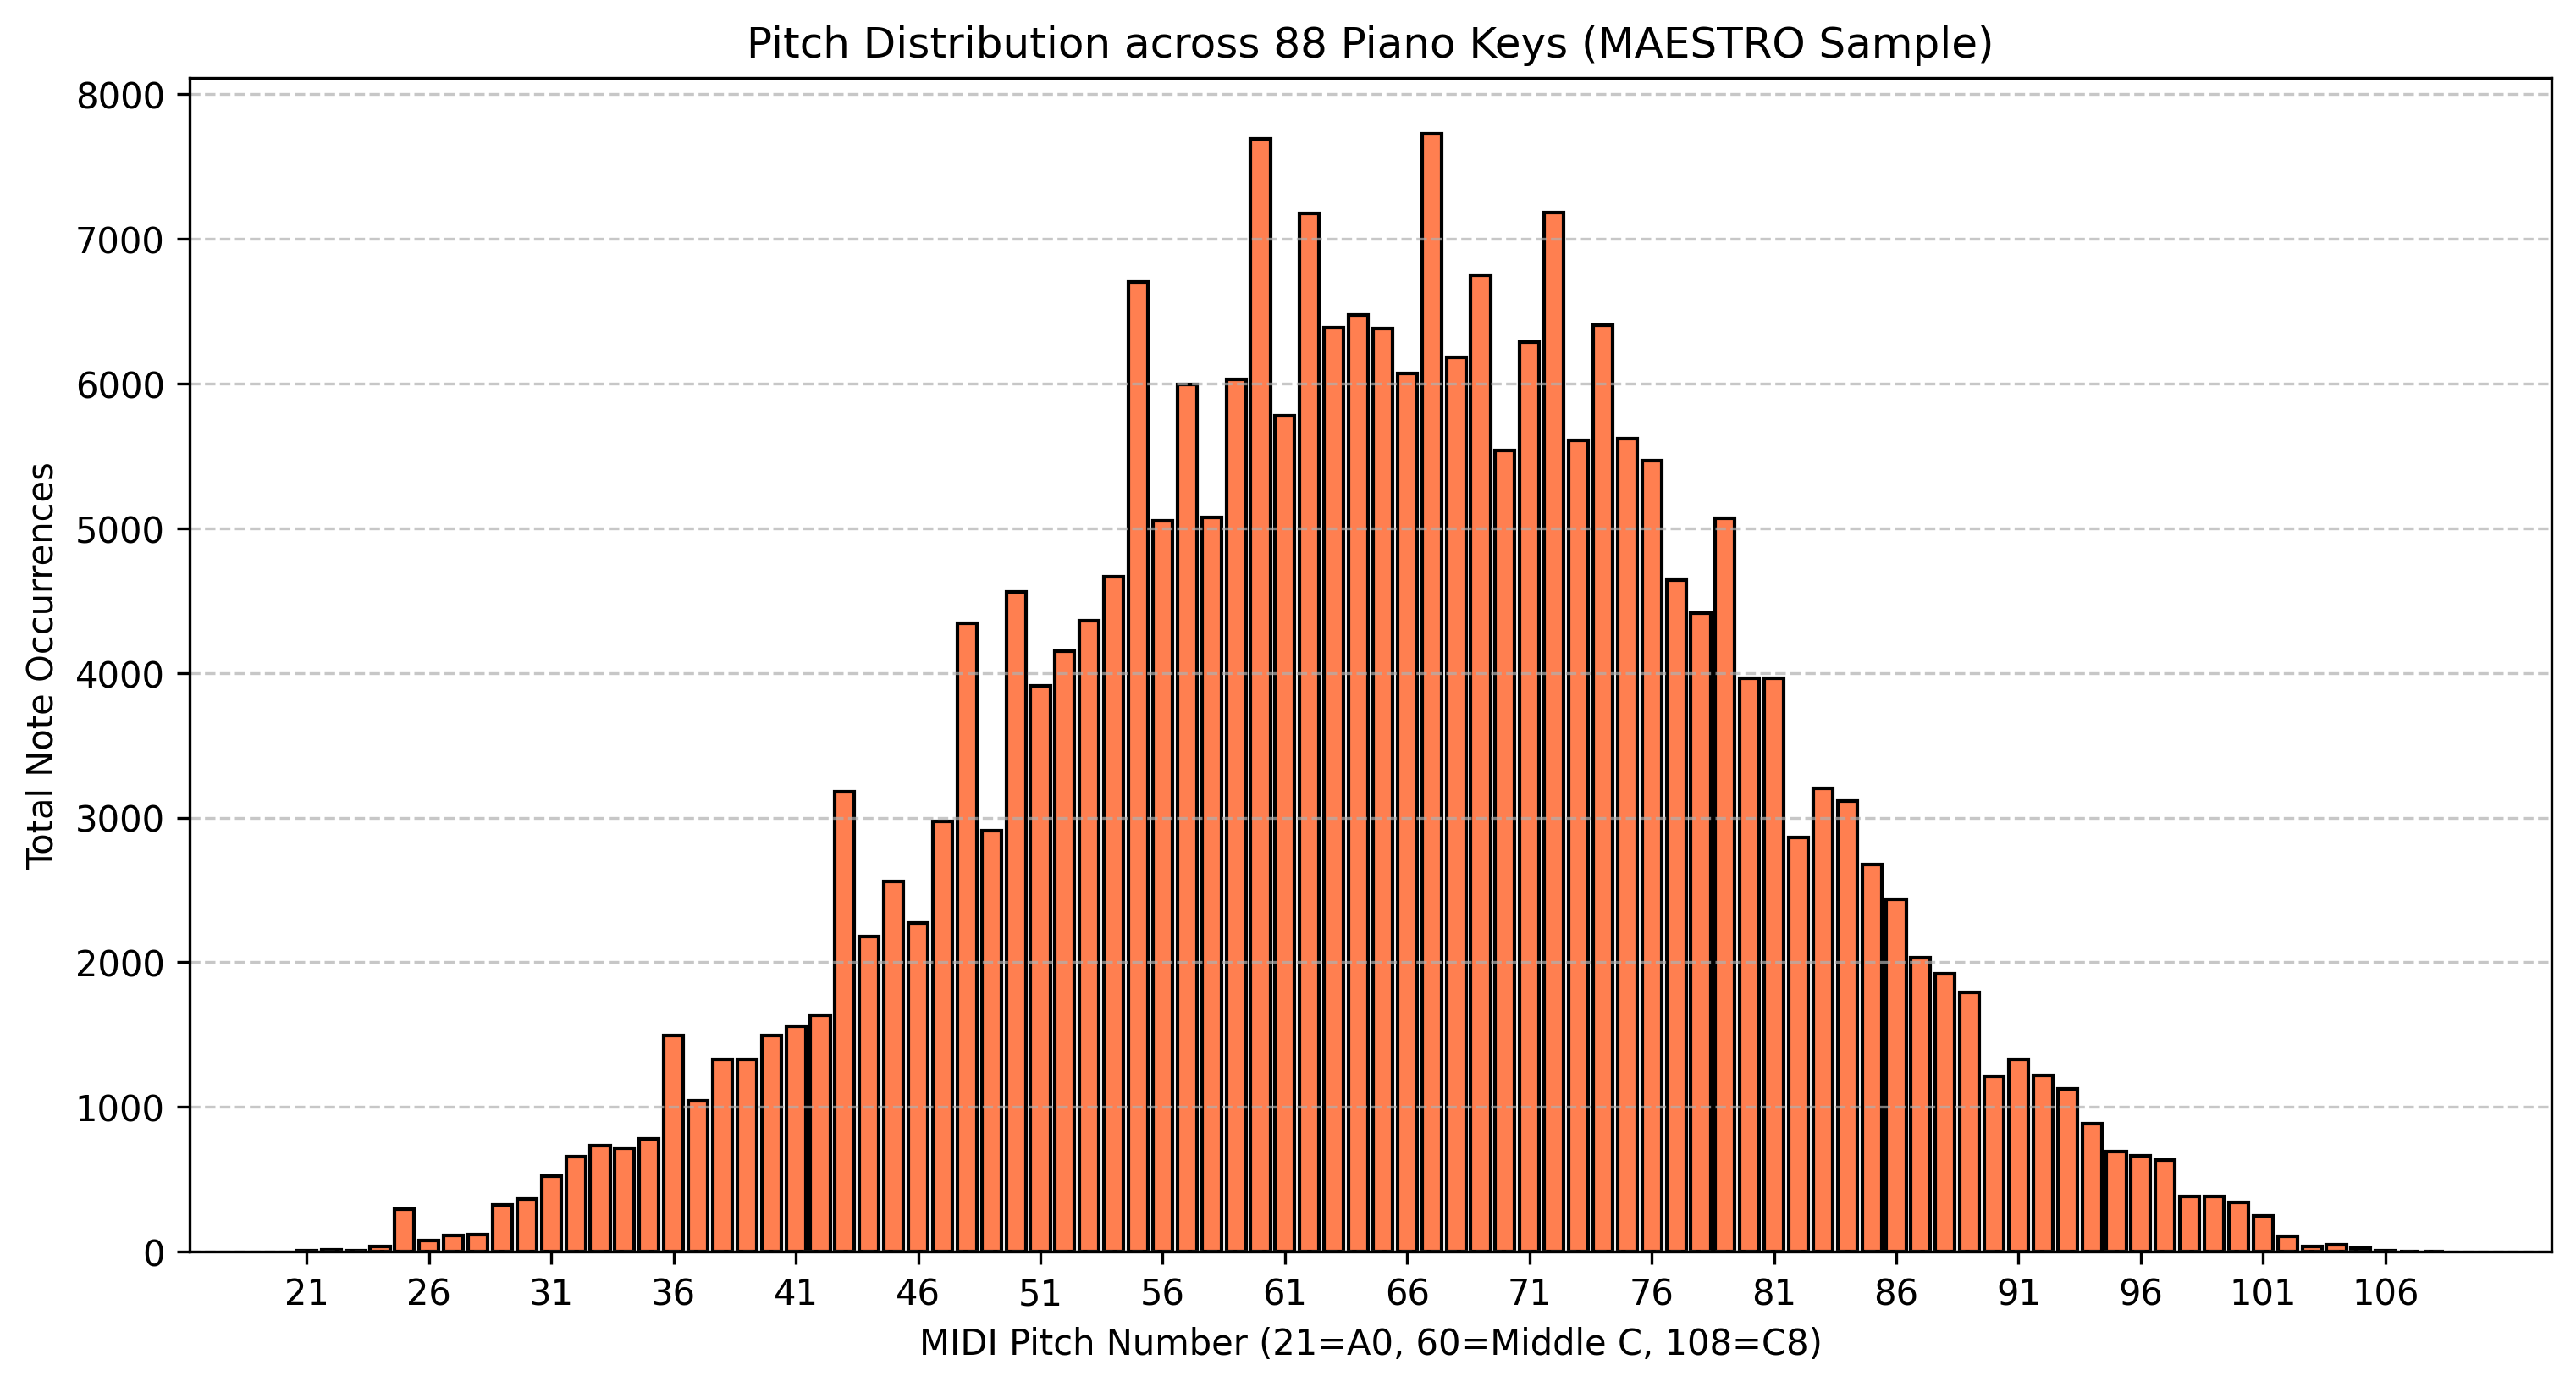
\includegraphics[width=1\linewidth]{images/eda_pitch_distribution.png}
    \caption{Pitch Distribution Analysis: Classical vs Modern Genres}
    \label{fig:task3_pitch}
\end{figure}

Qualitative assessment of the generated 1024-token sequences showed that the Transformer could maintain a consistent tempo and harmonic structure over several minutes, a feat that both the LSTM Autoencoder and VAE struggled with due to their fixed-window constraints. The use of REMI tokenization allowed the model to explicitly learn the relationship between note onsets and durations, leading to more natural phrasing.

\section{Conclusion}

This project demonstrated the progression of unsupervised neural networks for multi-genre music generation. We established that while LSTM Autoencoders and VAEs are efficient for local pattern compression and latent space exploration, they are inherently limited by sequence length and vanishing gradients. The introduction of the Transformer-based decoder, coupled with REMI tokenization and genre conditioning, proved to be the most effective solution for generating long, stylistically consistent musical compositions. Future work could involve extending this framework with Reinforcement Learning from Human Feedback (RLHF) to further refine the aesthetic quality and creativity of the generated pieces.



\bibliographystyle{icml2025}
\bibliography{example_paper}

\end{document}


% This document was modified from the file originally made available by
% Pat Langley and Andrea Danyluk for ICML-2K. This version was created
% by Iain Murray in 2018, and modified by Alexandre Bouchard in
% 2019 and 2021 and by Csaba Szepesvari, Gang Niu and Sivan Sabato in 2022.
% Modified again in 2023 and 2024 by Sivan Sabato and Jonathan Scarlett.
% Previous contributors include Dan Roy, Lise Getoor and Tobias
% Scheffer, which was slightly modified from the 2010 version by
% Thorsten Joachims & Johannes Fuernkranz, slightly modified from the
% 2009 version by Kiri Wagstaff and Sam Roweis's 2008 version, which is
% slightly modified from Prasad Tadepalli's 2007 version which is a
% lightly changed version of the previous year's version by Andrew
% Moore, which was in turn edited from those of Kristian Kersting and
% Codrina Lauth. Alex Smola contributed to the algorithmic style files.
